\documentclass[12pt,letterpaper]{article}
\usepackage[utf8]{inputenc}
\usepackage[spanish,es-noshorthands]{babel}
\usepackage{amsmath,amssymb}
\usepackage{graphicx}
\usepackage{xcolor}
\usepackage{tikz}
\usetikzlibrary{calc,arrows.meta,decorations.markings,patterns}
\usepackage[top=2.5cm, bottom=2.7cm, left=2cm, right=2cm, footskip=40pt]{geometry}
\usepackage{fancyhdr}
\usepackage{lastpage}

\definecolor{ubbblue}{RGB}{0,51,102}
\definecolor{cargazul}{RGB}{40,40,210}
\definecolor{cargarojo}{RGB}{210,40,40}

% separaci\'on vertical entre secciones
\newcommand{\secgap}{\vspace{0.55cm}}
% encabezado de cada problema
\newcommand{\problema}[1]{\noindent{\large\textcolor{ubbblue}{\textbf{#1}}}\par\smallskip}

\pagestyle{fancy}
\fancyhf{}
\renewcommand{\headrulewidth}{0pt}
\renewcommand{\footrulewidth}{0.4pt}
\fancyfoot[L]{\raisebox{-0.5\height}{
\includegraphics[height=1.1cm]{logo ubb.png}}}
\fancyfoot[C]{%
    \begin{minipage}[c]{8cm}\centering
        \footnotesize\textcolor{ubbblue}{\textbf{Dr.\ Arturo Fern\'andez P\'erez}}\\
        \scriptsize Departamento de F\'isica -- Universidad del B\'io-B\'io\\
        \scriptsize \textit{Electro\_Asistente\_AI-UBB}\\
        \tiny P\'agina \thepage\ de \pageref{LastPage}
    \end{minipage}}
\fancyfoot[R]{\raisebox{-0.5\height}{
\includegraphics[height=1.1cm]{logo dfis.png}}}
\fancypagestyle{plain}{%
    \fancyhf{}
    \renewcommand{\headrulewidth}{0pt}
    \renewcommand{\footrulewidth}{0.4pt}
    \fancyfoot[L]{\raisebox{-0.5\height}{
\includegraphics[height=1.1cm]{logo ubb.png}}}
    \fancyfoot[C]{%
        \begin{minipage}[c]{8cm}\centering
            \footnotesize\textcolor{ubbblue}{\textbf{Dr.\ Arturo Fern\'andez P\'erez}}\\
            \scriptsize Departamento de F\'isica -- Universidad del B\'io-B\'io\\
            \scriptsize \textit{Electro\_Asistente\_AI-UBB}\\
            \tiny P\'agina \thepage\ de \pageref{LastPage}
        \end{minipage}}
    \fancyfoot[R]{\raisebox{-0.5\height}{
\includegraphics[height=1.1cm]{logo dfis.png}}}
}

\begin{document}

\begin{center}
    
\includegraphics[height=2cm]{logo ubb.png}\\[0.3cm]
    {\large\textcolor{ubbblue}{\textbf{UNIVERSIDAD DEL B\'IO-B\'IO}}}\\[0.1cm]
    {\normalsize Facultad de Ciencias -- Departamento de F\'isica}
\end{center}

\vspace{0.3cm}\hrule height 1pt\vspace{0.5cm}

{\centering\Large\textbf{Pauta Tarea 1 \quad--\quad F\'isica II (2026-2)}\par}
{\centering\normalsize\textit{Fuerza y campo el\'ectrico: cargas puntuales y distribuciones continuas}\par}

\vspace{0.2cm}
{\centering\footnotesize $k=\dfrac{1}{4\pi\varepsilon_0}=9\times10^{9}\ \mathrm{N\,m^2/C^2}$\par}

\vspace{0.5cm}

%=====================================================================
% PROBLEMA 1
%=====================================================================
\problema{Problema 1. Fuerza sobre $q_3$ y campo en un punto del espacio}

\noindent Tres cargas puntuales $q_1=-3$ nC, $q_2=+2$ nC y $q_3=+5$ nC (Fig.~1).

\medskip
\noindent
\begin{minipage}[c]{0.40\textwidth}
\centering
\begin{tikzpicture}[scale=0.26, >=Stealth, line width=0.8pt]
    \draw[->,gray] (-11,0)--(11,0) node[right,font=\scriptsize]{$x$};
    \draw[->,gray] (0,-8.5)--(0,6.2) node[above,font=\scriptsize]{$y$};
    \node[gray,font=\tiny,above right] at (0.2,0.2){$O$};
    \filldraw[cargazul] (-8,5) circle (6pt);
    \node[cargazul,above,font=\scriptsize] at (-8,5.8){$q_2$};
    \filldraw[cargazul] (-10,-7) circle (6pt);
    \node[cargazul,below,font=\scriptsize] at (-10,-8){$q_3$};
    \filldraw[cargarojo] (10.39,-6) circle (6pt);
    \node[cargarojo,right,font=\scriptsize] at (10.9,-6){$q_1$};
    \draw[dashed,gray] (0,0)--(10.39,-6);
    \node[rotate=-30,font=\tiny] at (5.6,-2.6){$12$ cm};
    \draw (3.2,0) arc (0:-30:3.2);
    \node[font=\tiny] at (4.4,-1.1){$30^\circ$};
\end{tikzpicture}\\[1pt]
{\scriptsize \textbf{Figura 1} (cm)}
\end{minipage}%
\hfill
\begin{minipage}[c]{0.56\textwidth}
\textbf{Posiciones} (cm $\to$ m). $q_1$ est\'a a $12$ cm del origen, $30^\circ$ bajo el eje $x^+$:
\begin{align*}
\vec r_1&=(0{,}1039\,\hat\imath-0{,}06\,\hat\jmath)\ \mathrm{m},\\
\vec r_2&=(-0{,}08\,\hat\imath+0{,}05\,\hat\jmath)\ \mathrm{m},\\
\vec r_3&=(-0{,}10\,\hat\imath-0{,}07\,\hat\jmath)\ \mathrm{m}.
\end{align*}
Ley de Coulomb vectorial:
$\vec F_{ij}=k\,q_i q_j\,\dfrac{\vec r_i-\vec r_j}{\lVert\vec r_i-\vec r_j\rVert^{3}}$.
\end{minipage}

\secgap

\noindent\textbf{(a) Fuerza neta sobre $q_3$.} $\ \vec F_3=\vec F_{31}+\vec F_{32}$. Vectores relativos:
\[
\vec r_3-\vec r_1=(-0{,}2039\,\hat\imath-0{,}01\,\hat\jmath)\ \mathrm{m},\quad \lVert\vec r_3-\vec r_1\rVert=0{,}2042\ \mathrm{m},
\]
\[
\vec r_3-\vec r_2=(-0{,}02\,\hat\imath-0{,}12\,\hat\jmath)\ \mathrm{m},\quad \lVert\vec r_3-\vec r_2\rVert=0{,}1217\ \mathrm{m}.
\]
\begin{align*}
\vec F_{31}&=\frac{(9\times10^{9})(5\times10^{-9})(-3\times10^{-9})}{(0{,}2042)^{3}}\,(-0{,}2039\,\hat\imath-0{,}01\,\hat\jmath)
=(3{,}23\,\hat\imath+0{,}16\,\hat\jmath)\times10^{-6}\ \mathrm{N},\\[2pt]
\vec F_{32}&=\frac{(9\times10^{9})(5\times10^{-9})(2\times10^{-9})}{(0{,}1217)^{3}}\,(-0{,}02\,\hat\imath-0{,}12\,\hat\jmath)
=(-1{,}00\,\hat\imath-6{,}00\,\hat\jmath)\times10^{-6}\ \mathrm{N}.
\end{align*}
Superposici\'on por componentes:
\[
\boxed{\ \vec F_3=(2{,}24\,\hat\imath-5{,}84\,\hat\jmath)\times10^{-6}\ \mathrm{N},\qquad
\lVert\vec F_3\rVert=6{,}25\times10^{-6}\ \mathrm{N}\ }
\]

\secgap

\noindent\textbf{(b) Campo neto en $P=(2,-8,3)$ cm} $=(0{,}02\,\hat\imath-0{,}08\,\hat\jmath+0{,}03\,\hat k)$ m. \
Con $\vec E_j=k\,q_j\,\dfrac{\vec r_P-\vec r_j}{\lVert\vec r_P-\vec r_j\rVert^{3}}$:
\begin{align*}
\vec r_P-\vec r_1&=(-0{,}0839\,\hat\imath-0{,}02\,\hat\jmath+0{,}03\,\hat k),\quad \lVert\vec r_P-\vec r_1\rVert=0{,}0913;\\
\vec r_P-\vec r_2&=(0{,}10\,\hat\imath-0{,}13\,\hat\jmath+0{,}03\,\hat k),\quad \lVert\vec r_P-\vec r_2\rVert=0{,}1667;\\
\vec r_P-\vec r_3&=(0{,}12\,\hat\imath-0{,}01\,\hat\jmath+0{,}03\,\hat k),\quad \lVert\vec r_P-\vec r_3\rVert=0{,}1241\ \ \mathrm{(m)}.
\end{align*}
\begin{align*}
\vec E_1&=(2973\,\hat\imath+709\,\hat\jmath-1063\,\hat k),\quad
\vec E_2=(388\,\hat\imath-505\,\hat\jmath+117\,\hat k),\\[2pt]
\vec E_3&=(2826\,\hat\imath-235\,\hat\jmath+706\,\hat k)\qquad [\mathrm{N/C}].
\end{align*}
\[
\boxed{\ \vec E=(6187\,\hat\imath-32\,\hat\jmath-240\,\hat k)\ \mathrm{N/C},\qquad \lVert\vec E\rVert\approx 6{,}19\times10^{3}\ \mathrm{N/C}\ }
\]

\secgap

%=====================================================================
% PROBLEMA 2
%=====================================================================
\problema{Problema 2. Campo y fuerza en una configuraci\'on circular}

\noindent $q_1=q_2=3Q$, $q_3=-4Q$, con $Q=10\ \mu$C y $R=1{,}2$ m; la part\'icula $q_0=-Q$ est\'a en $P$ (Fig.~2). \
As\'i $q_1=q_2=30\ \mu$C, $q_3=-40\ \mu$C y $q_0=-10\ \mu$C.

\medskip
\noindent
\begin{minipage}[c]{0.34\textwidth}
\centering
\begin{tikzpicture}[scale=0.82, >=Stealth, line width=0.8pt]
    \draw[dashed,gray!70] (0,0) circle (2);
    \draw[->,gray] (-2.7,0)--(2.7,0) node[right,font=\scriptsize]{$x$};
    \draw[->,gray] (0,-2.7)--(0,2.7) node[above,font=\scriptsize]{$y$};
    \node[gray,font=\tiny,below left] at (0,0){$O$};
    \filldraw[cargazul] (90:2) circle (3.2pt);  \node[cargazul,above right,font=\scriptsize] at (90:2){$q_1$};
    \filldraw[cargazul] (0:2) circle (3.2pt);   \node[cargazul,above right,font=\scriptsize] at (0:2){$q_2$};
    \filldraw[cargarojo] (-50:2) circle (3.2pt); \node[cargarojo,below right,font=\scriptsize] at (-50:2){$q_3$};
    \filldraw[black] (180:2) circle (2.6pt);   \node[above left,font=\scriptsize] at (180:2){$P$};
    \draw[dotted,line width=1pt] (0,0)--(-50:2);
    \draw[->,gray] (0,0)--(58:2);
    \node[font=\scriptsize] at ($(58:1.2)+(0.3,0)$){$R$};
    \draw (0:0.75) arc (0:-50:0.75);
    \node[font=\tiny] at (-25:1.05){$50^\circ$};
\end{tikzpicture}\\[1pt]
{\scriptsize \textbf{Figura 2}}
\end{minipage}%
\hfill
\begin{minipage}[c]{0.62\textwidth}
\textbf{Posiciones} ($\lVert\cdot\rVert=R$ desde $O$):
\[
\vec r_1=(0\,\hat\imath+1{,}2\,\hat\jmath),\quad \vec r_2=(1{,}2\,\hat\imath),
\]
\[
\vec r_3=(0{,}771\,\hat\imath-0{,}919\,\hat\jmath),\quad \vec r_P=(-1{,}2\,\hat\imath)\ \ [\mathrm{m}].
\]
\textbf{L\'ineas de campo en $P$:} las cargas positivas $q_1,q_2$ \emph{repelen} (su campo en $P$ apunta \emph{alej\'andose} de ellas) y la negativa $q_3$ \emph{atrae} (su campo apunta \emph{hacia} $q_3$). El diagrama inferior muestra $\vec E_1,\vec E_2,\vec E_3$ y la resultante $\vec E_P$.
\end{minipage}

\secgap

\noindent\textbf{Campo neto en $P$.} Con $\vec E_j=k\,q_j\,\dfrac{\vec r_P-\vec r_j}{\lVert\vec r_P-\vec r_j\rVert^{3}}$:
\begin{align*}
\vec r_P-\vec r_1&=(-1{,}2\,\hat\imath-1{,}2\,\hat\jmath),\quad \lVert\vec r_P-\vec r_1\rVert=1{,}697\ \mathrm{m};\\
\vec r_P-\vec r_2&=(-2{,}4\,\hat\imath),\quad \lVert\vec r_P-\vec r_2\rVert=2{,}4\ \mathrm{m};\\
\vec r_P-\vec r_3&=(-1{,}971\,\hat\imath+0{,}919\,\hat\jmath),\quad \lVert\vec r_P-\vec r_3\rVert=2{,}175\ \mathrm{m}.
\end{align*}
\begin{align*}
\vec E_1&=\frac{(9\times10^{9})(30\times10^{-6})}{(1{,}697)^{3}}(-1{,}2\,\hat\imath-1{,}2\,\hat\jmath)=(-6{,}63\,\hat\imath-6{,}63\,\hat\jmath)\times10^{4},\\[2pt]
\vec E_2&=\frac{(9\times10^{9})(30\times10^{-6})}{(2{,}4)^{3}}(-2{,}4\,\hat\imath)=(-4{,}69\,\hat\imath)\times10^{4},\\[2pt]
\vec E_3&=\frac{(9\times10^{9})(-40\times10^{-6})}{(2{,}175)^{3}}(-1{,}971\,\hat\imath+0{,}919\,\hat\jmath)=(6{,}90\,\hat\imath-3{,}22\,\hat\jmath)\times10^{4}\quad[\mathrm{N/C}].
\end{align*}
\[
\boxed{\ \vec E_P=(-4{,}42\,\hat\imath-9{,}84\,\hat\jmath)\times10^{4}\ \mathrm{N/C},\qquad \lVert\vec E_P\rVert=1{,}08\times10^{5}\ \mathrm{N/C}\ }
\]

\smallskip
\begin{center}
\begin{tikzpicture}[scale=1.0, >=Stealth, line width=0.9pt]
    \filldraw[black] (0,0) circle (1.6pt); \node[below,font=\scriptsize] at (0,-0.08){$P$};
    % E1 (down-left, 225 aprox) escala reducida
    \draw[->,cargazul] (0,0)--(-1.02,-1.02); \node[cargazul,font=\scriptsize,above left] at (-1.02,-1.02){$\vec E_1$};
    % E2 (left, 180)
    \draw[->,cargazul] (0,0)--(-1.10,0); \node[cargazul,font=\scriptsize,above] at (-1.15,0.05){$\vec E_2$};
    % E3 (right-down, -25)
    \draw[->,cargarojo] (0,0)--(1.30,-0.60); \node[cargarojo,font=\scriptsize,right] at (1.30,-0.60){$\vec E_3$};
    % resultante EP (down-left, -114)
    \draw[->,black,line width=1.3pt] (0,0)--(-0.62,-1.38); \node[font=\scriptsize,below left] at (-0.62,-1.38){$\vec E_P$};
\end{tikzpicture}\\[-2pt]
{\scriptsize L\'ineas/vectores de campo en $P$ (no a escala).}
\end{center}

\secgap

\noindent\textbf{Fuerza sobre $q_0=-Q$.} Como $q_0<0$, $\vec F_0=q_0\vec E_P$ apunta en sentido \emph{opuesto} a $\vec E_P$:
\[
\boxed{\ \vec F_0=q_0\vec E_P=(0{,}44\,\hat\imath+0{,}98\,\hat\jmath)\ \mathrm{N},\qquad \lVert\vec F_0\rVert=1{,}08\ \mathrm{N}\ }
\]

\secgap

%=====================================================================
% PROBLEMA 3
%=====================================================================
\problema{Problema 3. Barra finita sobre el eje $y$}

\noindent Barra con $\lambda=-8{,}5$ nC/m uniforme sobre el eje $y$, entre $y=5$ y $y=18$ cm; carga $q=+16$ nC en $P=(5,-7)$ cm (Fig.~3).

\medskip
\noindent
\begin{minipage}[c]{0.30\textwidth}
\centering
\begin{tikzpicture}[scale=0.20, >=Stealth, line width=0.8pt]
    \draw[->,gray] (-3,0)--(8,0) node[right,font=\scriptsize]{$x$};
    \draw[->,gray] (0,-9.5)--(0,20.5) node[above,font=\scriptsize]{$y$};
    \node[gray,font=\tiny,below left] at (0,0){$O$};
    \draw[cargarojo,line width=3pt] (0,5)--(0,18);
    \node[cargarojo,right,font=\scriptsize] at (0.7,11.5){$\lambda$};
    \draw[gray] (-0.6,5)--(0.6,5);   \node[font=\tiny,left] at (-0.8,5){$y{=}5$};
    \draw[gray] (-0.6,18)--(0.6,18); \node[font=\tiny,left] at (-0.8,18){$y{=}18$};
    \draw[dashed,gray] (0,-7)--(5,-7); \draw[dashed,gray] (5,0)--(5,-7);
    \filldraw[cargazul] (5,-7) circle (5pt);
    \node[cargazul,right,font=\scriptsize] at (5.8,-7){$q$};
    \node[font=\tiny,below] at (5,-8.6){$P(5,-7)$};
\end{tikzpicture}\\[1pt]
{\scriptsize \textbf{Figura 3} (cm)}
\end{minipage}%
\hfill
\begin{minipage}[c]{0.66\textwidth}
\textbf{Elemento y vector posici\'on.} Un elemento $dq=\lambda\,dy'$ en $\vec r\,'=(0,y')$ produce en $P=(0{,}05,-0{,}07)$:
\begin{align*}
\vec r_P-\vec r\,'&=\big(0{,}05\,\hat\imath-(0{,}07+y')\,\hat\jmath\big),\\
\lVert\vec r_P-\vec r\,'\rVert&=\sqrt{0{,}05^2+(0{,}07+y')^2}.
\end{align*}
\[
\vec E=k\lambda\!\int_{0{,}05}^{0{,}18}\!\frac{0{,}05\,\hat\imath-(0{,}07+y')\,\hat\jmath}{\big(0{,}05^2+(0{,}07+y')^2\big)^{3/2}}\,dy'.
\]
\end{minipage}

\secgap

\noindent Con la sustituci\'on $u=y'+0{,}07$ ($u:0{,}12\to0{,}25$) las integrales tienen forma cerrada:
\begin{align*}
E_x&=k\lambda(0{,}05)\left[\frac{u}{0{,}05^2\sqrt{0{,}05^2+u^2}}\right]_{0{,}12}^{0{,}25}=-88{,}0\ \mathrm{N/C},\\[2pt]
E_y&=k\lambda\left[\frac{1}{\sqrt{0{,}05^2+u^2}}\right]_{0{,}12}^{0{,}25}=+288{,}4\ \mathrm{N/C}.
\end{align*}
El campo apunta \emph{hacia} la barra (carga negativa, atractiva sobre una prueba positiva):
\[
\boxed{\ \vec E=(-88{,}0\,\hat\imath+288{,}4\,\hat\jmath)\ \mathrm{N/C},\qquad \lVert\vec E\rVert=301{,}5\ \mathrm{N/C}\ }
\]
Fuerza sobre $q=+16$ nC (mismo sentido que $\vec E$):
\[
\boxed{\ \vec F=q\vec E=(-1{,}41\,\hat\imath+4{,}61\,\hat\jmath)\times10^{-6}\ \mathrm{N},\qquad \lVert\vec F\rVert=4{,}82\times10^{-6}\ \mathrm{N}\ }
\]

\secgap

%=====================================================================
% PROBLEMA 4
%=====================================================================
\problema{Problema 4. Segmento de circunferencia (campo en el eje)}

\noindent Arco de radio $R=15$ cm, entre $\phi_1=\frac{5\pi}{6}$ y $\phi_2=\frac{4\pi}{3}$ (desde $x^+$), con $\lambda=4{,}0\ \mu$C/m. Punto $P$ en el eje $z$, a $z_0=8$ cm del centro (Fig.~4); luego $q=7{,}0\ \mu$C en $P$.

\medskip
\noindent
\begin{minipage}[c]{0.32\textwidth}
\centering
\begin{tikzpicture}[scale=0.9, >=Stealth, line width=0.8pt,
    x={(-0.52cm,-0.36cm)}, y={(1cm,0cm)}, z={(0cm,1cm)}]
    \draw[->,gray] (0,0,0)--(2.3,0,0) node[below,font=\scriptsize]{$x$};
    \draw[->,gray] (0,0,0)--(0,2.3,0) node[right,font=\scriptsize]{$y$};
    \draw[->,gray] (0,0,0)--(0,0,2.6) node[above,font=\scriptsize]{$z$};
    \draw[cargazul,line width=1.9pt]
        plot[domain=150:240,samples=50,variable=\t] ({1.6*cos(\t)},{1.6*sin(\t)},0);
    \node[cargazul,font=\scriptsize] at ({2.0*cos(196)},{2.0*sin(196)},0.12){$\lambda$};
    \draw[dashed,gray] (0,0,0)--({1.6*cos(150)},{1.6*sin(150)},0);
    \node[font=\tiny] at ({1.86*cos(150)},{1.86*sin(150)},0.12){$\phi_1$};
    \draw[dashed,gray] (0,0,0)--({1.6*cos(240)},{1.6*sin(240)},0);
    \node[font=\tiny] at ({1.83*cos(240)},{1.83*sin(240)},0.12){$\phi_2$};
    \node[font=\tiny] at ({0.9*cos(150)},{0.9*sin(150)},0.22){$R$};
    \draw[dashed,gray] (0,0,0)--(0,0,1.8);
    \filldraw[black] (0,0,1.8) circle (1.8pt);
    \node[right,font=\scriptsize] at (0,0.08,1.8){$P$};
    \node[font=\tiny,left] at (0,-0.05,1.0){$z_0$};
\end{tikzpicture}\\[1pt]
{\scriptsize \textbf{Figura 4}}
\end{minipage}%
\hfill
\begin{minipage}[c]{0.64\textwidth}
\textbf{Elemento y posiciones.} $dq=\lambda\,ds=\lambda R\,d\phi$ en $\vec r_q=(R\cos\phi,R\,\mathrm{sen}\,\phi,0)$; con $\vec r_P=z_0\hat k$:
\[
\vec r_P-\vec r_q=(-R\cos\phi\,\hat\imath-R\,\mathrm{sen}\,\phi\,\hat\jmath+z_0\hat k),
\]
\[
\lVert\vec r_P-\vec r_q\rVert=\sqrt{R^2+z_0^2}=0{,}17\ \mathrm{m}\ \ (\text{indep.\ de }\phi).
\]
Como $\sqrt{R^2+z_0^2}$ es constante, sale de la integral.
\end{minipage}

\secgap

\noindent Integrando $\phi$ de $\tfrac{5\pi}{6}$ a $\tfrac{4\pi}{3}$ (con $(R^2+z_0^2)^{3/2}=4{,}913\times10^{-3}$):
\begin{align*}
E_x&=\frac{-k\lambda R^2}{(R^2+z_0^2)^{3/2}}\big(\mathrm{sen}\,\phi_2-\mathrm{sen}\,\phi_1\big)
   =\frac{-(9\times10^{9})(4\times10^{-6})(0{,}15)^2}{4{,}913\times10^{-3}}(-1{,}366)=2{,}25\times10^{5},\\[2pt]
E_y&=\frac{-k\lambda R^2}{(R^2+z_0^2)^{3/2}}\big(-\cos\phi_2+\cos\phi_1\big)
   =(1{,}649\times10^{5})(-1)(-0{,}366)=6{,}03\times10^{4},\\[2pt]
E_z&=\frac{k\lambda R\,z_0}{(R^2+z_0^2)^{3/2}}\,(\phi_2-\phi_1)
   =\frac{(9\times10^{9})(4\times10^{-6})(0{,}15)(0{,}08)}{4{,}913\times10^{-3}}\cdot\frac{\pi}{2}=1{,}38\times10^{5}\quad[\mathrm{N/C}].
\end{align*}
\[
\boxed{\ \vec E=(2{,}25\times10^{5}\,\hat\imath+6{,}03\times10^{4}\,\hat\jmath+1{,}38\times10^{5}\,\hat k)\ \mathrm{N/C},\qquad \lVert\vec E\rVert=2{,}71\times10^{5}\ \mathrm{N/C}\ }
\]
Fuerza sobre $q=7{,}0\ \mu$C:
\[
\boxed{\ \vec F=q\vec E=(1{,}58\,\hat\imath+0{,}42\,\hat\jmath+0{,}97\,\hat k)\ \mathrm{N},\qquad \lVert\vec F\rVert=1{,}90\ \mathrm{N}\ }
\]

\secgap

%=====================================================================
% PROBLEMA 5
%=====================================================================
\problema{Problema 5. Semicircunferencia y segmento recto (campo en $O$)}

\noindent La l\'inea 1 es una \emph{semicircunferencia} de radio $R$ (semiplano superior, $\phi:0\to\pi$) con $\lambda_1=-18\ \mu$C/m. La l\'inea 2 es un \emph{segmento recto} sobre el eje $y$, de largo $R$, entre $y=-R$ e $y=-2R$, con carga total $Q_2=70\ \mu$C. $R=20$ cm (Fig.~5).

\medskip
\noindent
\begin{minipage}[c]{0.30\textwidth}
\centering
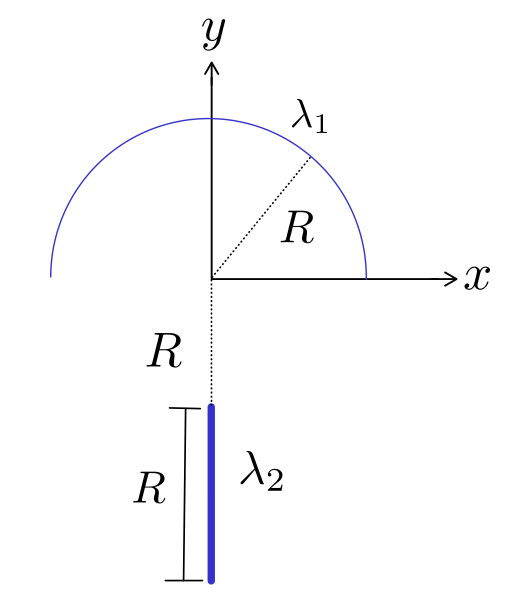
\includegraphics[width=4.6cm]{Electro1.png}\\[1pt]
{\scriptsize \textbf{Figura 5}}
\end{minipage}%
\hfill
\begin{minipage}[c]{0.66\textwidth}
\textbf{(a) Densidad y carga.} La l\'inea 2 (largo $R$): $\ \lambda_2=\dfrac{Q_2}{R}=\dfrac{70\ \mu\mathrm{C}}{0{,}20\ \mathrm{m}}$. \
La l\'inea 1 (largo $\pi R$): $\ Q_1=\lambda_1(\pi R)$.
\[
\boxed{\ \lambda_2=350\ \mu\mathrm{C/m}\ };\qquad \boxed{\ Q_1=-11{,}3\ \mu\mathrm{C}\ }
\]
\end{minipage}

\secgap

\noindent\textbf{(b) Campo $\vec E_1$ de la semicircunferencia en $O$.} $dq=\lambda_1 R\,d\phi$ en $\vec r_q=(R\cos\phi,R\,\mathrm{sen}\,\phi)$; $\vec r_O-\vec r_q=(-R\cos\phi,-R\,\mathrm{sen}\,\phi)$ con $\lVert\vec r_O-\vec r_q\rVert=R$:
\[
\vec E_1=\frac{k\lambda_1}{R}\!\int_{0}^{\pi}(-\cos\phi\,\hat\imath-\mathrm{sen}\,\phi\,\hat\jmath)\,d\phi
=\frac{k\lambda_1}{R}\big(0\,\hat\imath-2\,\hat\jmath\big)=-\frac{2k\lambda_1}{R}\,\hat\jmath.
\]
Con $\lambda_1<0$ el campo apunta hacia la carga ($+\hat\jmath$):
\[
\boxed{\ \vec E_1=+1{,}62\times10^{6}\,\hat\jmath\ \mathrm{N/C}\ }
\]

\secgap

\noindent\textbf{(c) Campo $\vec E_2$ del segmento en $O$.} $dq=\lambda_2\,dy'$ en $\vec r_q=(0,y')$, $y'\in[-2R,-R]$; $\vec r_O-\vec r_q=(0,-y')$, $\lVert\cdot\rVert=|y'|$:
\[
\vec E_2=k\lambda_2\!\int_{-2R}^{-R}\frac{-y'}{|y'|^{3}}\,dy'\ \hat\jmath
=k\lambda_2\!\left[\frac{1}{R}-\frac{1}{2R}\right]\hat\jmath=\frac{k\lambda_2}{2R}\,\hat\jmath.
\]
\[
\boxed{\ \vec E_2=+7{,}88\times10^{6}\,\hat\jmath\ \mathrm{N/C}\ }
\]

\secgap

\noindent\textbf{(d) Campo neto en $O$.} Ambos aportes son axiales ($+\hat\jmath$):
\[
\boxed{\ \vec E_T=\vec E_1+\vec E_2=+9{,}50\times10^{6}\,\hat\jmath\ \mathrm{N/C}\ }
\]

\end{document}
